\documentclass[a4paper,10pt]{article}
\usepackage[utf8]{inputenc}
\usepackage[english]{babel}
\usepackage{graphics}
\usepackage{graphicx} %per le figure
\usepackage{subfigure} %per le figure
\usepackage{multirow}
\usepackage{geometry}
\usepackage{pdfpages}
\usepackage{esvect}
\usepackage{tikz,amsmath}
\usepackage{hyperref}
\usepackage{pdfpages}
\usepackage{xintexpr}
\usepackage{calc} 
\usepackage{forloop}

% This computes first argument as result of evaluation of second
% argument.
\newcommand*{\bind}[2]{\xintdefvar #1:=#2;\xinttheexpr #1\relax}

% The first argument specifies the number of digits
% to retain for fixed point output after decimal mark
% Default is 0, which means, round to nearest integer.
\newcommand*{\use}[2][0]{\xinttheiexpr [#1]#2\relax} 

\newcounter{counter}


\newcommand{\decay}{$\omega \rightarrow \pi^+ \pi^- \pi^0$ }
\newcommand{\production}{$\gamma p \rightarrow p \omega$ }
\newcommand{\fullreaction}{$\gamma p \rightarrow p \omega \rightarrow p \pi^+ \pi^- \pi^{0}$ }

\newtheorem{theorem}{Theorem}
\newcommand{\printteolike}{
Assume that, in an extended maximum likelihood fit, the intensity $I$ can be written as $I=I_1(\tau_1) \cdot I_2(\tau_2,\vec{x})$,
where the first factor does not include free parameters. Then, the likelihood obtained from the full intensity $I$ is equivalent to the
likelihood obtained by considering the $I_2$ factor only, provided that a weight $k_i$ is assigned to each of the MonteCarlo events -generated and reconstructed -, with $k_i=I_1(\tau^i_1)$, and that the average number of measured events is computed as:
\begin{equation}
\mu(\vec{x})=\frac{\sum_{i=1}^{N_{acc}}k_iI_2(\tau_2,\vec{x})}{N_{gen}}
\end{equation}
}


\author{Andrea Celentano\thanks{andrea.celentano@ge.infn.it}\\ \small{INFN, Sezione di Genova}}
\title{Analysis of the decay \decay with an extended Veneziano model}
\begin{document}
\maketitle
\begin{abstract}
In this note I describe the analysis of the decay \decay performed using an extended Veneziano model.
The main goal of the analysis is to verify that the model is able to correctly describe the data, and to determine the corresponding free parameters (the Regge trajectory parameters) trough a maximum likelihood fit.
From these, the $\rho$ meson pole parameters are obtained and compared to the corresponding PDG values.
Data were collected during the $g11a$ run, by measuring the photo-production reaction \production in the energy range $2.0< W < 2.45$ GeV. 

\end{abstract}
\tableofcontents
\section{Introduction}
In this note I describe the analysis of the decay \decay performed using the extended Veneziano model developed by A.~Sczepaniak in \cite{Szczepaniak:2014qca}, described in Section~\ref{sec:model}.
The amplitude employed to fit the data is constructed starting from a set of covariant Veneziano terms, resulting to a finite sum of partial waves that receive contributions from selected Regge trajectories, including the daughters, while still keeping the
proper asymptotic limit. Given the phase-space available to the \decay decay process, data sensitivity is limited to the first $\pi \pi$ Regge trajectory, containing the $\rho(770$) pole. For this reason, the simple, linear parametrization of the real part of the Regge trajectory was employed. The imaginary
part, instead, was ``ad-hoc'' tuned to reproduce the finite $\rho$ width.

The data were collected at Jefferson Lab, using the CLAS detector, as part of the g11a run period in 2004. 
This data has been already analyzed by Mike~Williams to extract the differential $\omega$ photo-production cross-section $\frac{d\sigma}{dt}$
and the $\omega$ spin density matrix elements $\rho_{00}$, $\rho_{1-1}$, $Re(\rho_{10})$, in the $\sqrt{s}$ range  from threshold up to 2.84 GeV \cite{Williams:2009ab}. 
Unfortunately, the already-processed data, and the corresponding analysis tools, were lost few years ago when one of the raid disks at CMU crashed and was unable to be recovered \cite{BrianCommunication}.

The data employed in this analysis comes from Brian~Vernansky PhD thesis.
As a ``preliminary'' part of his work, Brian re-processed the original g11a data-set, starting from ``cooked'' data, to extract the above observables,
in order to tune the analysis tools and procedures that he later employed in the analysis of the g1c and g8b data. He strictly followed the original analysis procedure from Mike Williams, described in 
\cite{Williams:thesis}, i.e. he applied to the cooked data the same set of selection cuts and corrections.

The input for this analysis are the fully reconstructed 4-vectors for the particles in the reaction \fullreaction, associated, event-by-event, 
to a weight (``Q-value''), that gives the probability for each event to originate from the signal distribution \cite{Williams:2008ac}. 
Brian also provided me a large set of MonteCarlo events, generated according to a pure phase-space distribution, projected on the CLAS detector and then reconstructed using the ``standard'' CLAS procedures. 


\section{\decay decay distribution}
In this section, I describe the general features of the \decay decay distribution, with the $\omega$ produced in the reaction \production.
I work in the ``Adair'' reference frame, defined as the $\omega$ rest frame, with the $z$ axis oriented along the photon momentum in the overall CM frame, and the scattered proton momentum lying in the $x-z$ plane.

Five independent kinematic variables are necessary to describe this process. The orientation of the normal to the decay plane, $\hat{n}_D$, is defined by the two angles $\theta_A$ and $\phi_A$, while two more variables completely fix the kinematics
of the pions on the decay plane. For these, one can use two of the three pion pairs invariant masses, related by:
\begin{equation}
M_W^2-m^2_{\pi^+} -m^2_{\pi^-} - m^2_{\pi^0} = s + t + u \; \; \; ,
\end{equation}
where $s=m^2_{\pi^+ \pi^0}$, $t=m^2_{\pi^0 \pi^-}$, $u=m^2_{\pi^+ \pi^-}$ are the pion pair invariant masses squared. Finally, the last kinematic variable corresponds to an overall rotation around the $z$ axis: since neither the photon beam or the proton target are polarized,
this rotation angle does not appear in the \decay decay distribution, and will be neglected.

\subsection{General features of the \decay decay distribution}

The general decay amplitude for the process $\omega \rightarrow \pi^+ \pi^- \pi^0$ follows directly from the $1^{--}$ nature of the $\omega$ meson:
\begin{equation}
A_{\lambda}=[(\vec{I}_{\pi^+} \times \vec{I}_{\pi^-})\cdot \vec{I}_{\pi^0}] \, \cdot \, \varepsilon_{\mu \nu \alpha \beta}\, p^{\nu}_{+}p^{\alpha}_{-}p^{\beta}_{0}\varepsilon^{\mu}_{\lambda} \, F(s,t,u)  \; \; \; ,
\end{equation}
where:
\begin{itemize}
\item $p_{+,0,-}$ are the pions 4-momenta
\item $\varepsilon_{\lambda}$ is the omega polarization four-vector, for the polarization $\lambda$ ($\lambda=-1,0,1$).
\item The isosospin factor $(\vec{I}_{\pi^+} \times \vec{I}_{\pi^-})\cdot \vec{I}_{\pi^0}$ contributes with a constant phase $i$ to the amplitude, and, therefore, can be neglected.
\item $\varepsilon_{\mu \nu \alpha \beta}$ is the Levi-Civita tensor
\item $F(s,t,u)$ is a general scalar function of Lorentz-invariant Dalitz variables (i.e. the pion pairs invariant masses squared).
\end{itemize}

I explicitely evaluate this in the Adair frame, where $p_+ + p_- + p_0 = (M_W;\vec{0})$. This gives:
\begin{equation}
A_{\lambda}=\varepsilon_{\mu \nu \alpha 0} M_{\omega} p^{\nu}_{+}p^{\alpha}_{-}\varepsilon^{\mu}_{\lambda} \cdot F(s,t,u)
=
M_{\omega}\cdot F(s,t,u)\cdot (\vec{p}_{+}\times\vec{p}_{-})\cdot \vec{\varepsilon}_{\lambda}
\end{equation}

The corresponding decay intensity is obtained by squaring the amplitude and inserting the $\omega$ polarization matrix $\rho^\omega_{\lambda,\lambda^\prime}$ (see \cite{Schilling:1969um}, Eq.~6):

\begin{eqnarray}
I&=&\sum_{\lambda,\lambda^\prime} A^*_{\lambda} \rho^\omega_{\lambda,\lambda^\prime} A_{\lambda^\prime}\\
I&=&M^2_\omega \cdot |F(s,t,u)|^2 \cdot \sum_{\lambda,\lambda^\prime} (\vec{p}_{+}\times\vec{p}_{-})\cdot \vec{\varepsilon}^*_{\lambda} \rho^\omega_{\lambda,\lambda^\prime} (\vec{p}_{+}\times\vec{p}_{-})\cdot \vec{\varepsilon}_{\lambda^\prime}
\end{eqnarray}
The vector product $\vec{p}_{+}\times\vec{p}_{-}$ is, by definition, orthogonal to the decay plane, and, therefore, can be written as $\hat{n}_D \cdot q$, with $q\equiv | \vec{p}_{+}\times\vec{p}_{-} |$.
Furthermore, which of the 3 pions 3-momenta are used in the calculation, and in which order, is irrelevant, since $\vec{p}_{+}+\vec{p}_{-}+\vec{p}_{0}=\vec{0}$ in Adair frame.

The intensity, therefore, reads:
\begin{equation}
I=q^2M^2_\omega \cdot |F(s,t,u)|^2 \cdot \sum_{\lambda,\lambda^\prime} \hat{n}_D\cdot \vec{\varepsilon}^*_{\lambda} \, \rho^\omega_{\lambda,\lambda^\prime} \, \hat{n}_D\cdot \vec{\varepsilon}_{\lambda^\prime}
\end{equation}
By elaborating this expression with the explicit form of $\varepsilon_\lambda$ and $\hat{n}_D$ one gets:
\begin{equation}\label{eq:intensity}
I=q^2M^2_\omega \cdot |F(s,t,u)|^2 \cdot W(\theta_A, \phi_A, \rho^\omega) \; \; \;,
\end{equation}
where $W(\theta_A,\phi_A,\rho^\omega)$ is given in \cite{Schilling:1969um}, Eq. 10. $W(\theta_A,\phi_A,\rho^\omega)$ gives the angular distribution of the $\omega$ decay plane. 
Since the $\omega$ meson is produced in the \production process, 
there is a direct relation between the $\omega$ polarization matrix and the incident photon polarization matrix
 in terms of the corresponding production amplitude $T$  (\cite{Schilling:1969um}, Eq.~2 and 3):
\begin{equation}\label{eq:rho}
\rho^\omega=T \, \rho^\gamma \, T^\dagger \; \; \;
\end{equation}
In case of unpolarized photon beam, this permits to simplify $W$ to:
\begin{equation}
W(\theta_A,\phi_A) = (\frac{1}{2}(1-\rho_{00})+\frac{1}{2}(3\rho_{00}-1)\cos^2\theta_A -\sqrt{2}Re(\rho_{10})\sin2\theta_A \cos\phi_A -\rho^0_{1-1} \sin^{2}\theta_A \cos 2\phi_A)
\end{equation}

Here, $\rho_{00}$, $Re(\rho_{10})$ and $\rho^0_{1-1}$ are the $\omega$ spin-density matrix elements relevant for the unpolarized beam, unpolarized target case. They do explicitely depend on the production kinematic variables ($W$ and $\cos\theta_{CM}$), 
as shown excplicitely by Eq.~\ref{eq:rho}. For the kinematic range covered in this analysis, these spin-density matrix elements, together with the differential production cross-section, have been already measured \cite{Williams:2009ab}.

The $\omega$ decay intensity, reported in Eq.~\ref{eq:intensity}, shows a complete factorization between the angular variables $\theta_A,\phi_A$ and the Dalitz variables $s,t,u$: 
this permits to simplify the maximum likelihood fit procedure, focusing only on the Dalitz part, as explained later in Sec.~\ref{sec:fitprocedure}.

\subsection{Extended Veneziano Model}\label{sec:model}


\section{\decay : extended maximum likelihood fit procedure}\label{sec:fitprocedure}

In this section, I describe the procedure that I adopted to fit the extended Veneziano model to the \decay decay, via an extended maximum likelihood fit.
In particular, I discuss what is the role of the production kinematic variables ($W$ and $\cos\theta_{CM}$) and observables (differential cross section and spin-density matrix elements).

\subsection{Extended maximum likelihood fits}

The goal of an extended maximum likelihood procedure is to fit a parametrized intensity for a certain reaction to a set of unbinned data, in order to extract the value of the corresponding free parameters and obtain 
the acceptance-corrected event yield. The intensity normalization is always a free parameter in the fit.

The main quantity of interest is the \textit{likelihood} $\mathcal L$, defined as the product of the occurrence probabilities of the measured events, according to the model used to derive the process intensity:
\begin{equation}\label{eq:PWA_TEO-1}
\mathcal L=\prod_i^n P_i(\tau_i,\vec{x}) \; ,
\end{equation} 
where the product is extended over all the $n$ measured events, each described by a set of kinematic variables $\tau_i$, and $\vec{x}$ are the parameters to be extracted from the data. For each event, the probability is proportional to the intensity multiplied by the detector acceptance $\varepsilon$, which in turns is a function of the final state kinematic variables:
\begin{equation}\label{eq:PWA_TEO-2}
P_i(\tau_i,\vec{x}) \propto I(\tau_i,\vec{x}) \cdot \varepsilon(\tau_i)
\end{equation}
The overall normalization is fixed requiring that the integral of the intensity multiplied by the detector acceptance, over the full final state phase space, is equal to the average number of expected events $\mu$:
\begin{eqnarray}\label{eq:PWA_TEO-3}
\mu(\vec{x})&=&\int I(\tau,\vec{x}) \cdot \varepsilon(\tau) d\tau \;  \\
P_i(\tau_i,\vec{x}) &=&\frac{ I(\tau_i,\vec{x}) \cdot \varepsilon(\tau_i) } {\int I(\tau,\vec{x}) \cdot \varepsilon(\tau) d\tau}
\end{eqnarray}
The total number of measured events $n$ itself is a statistical variable, distributed according to the Poisson statistics. A proper factor accounting for the probability to measure \textit{exactly} $n$ events has thus to be introduced into the likelihood expression, getting its final expression:
\begin{equation}\label{eq:PWA_TEO-4}
\mathcal L=\frac{\mu^{n}e^{-\mu}}{n!}\cdot \prod_i^n \frac{ I(\tau_i,\vec{x}) \cdot \varepsilon(\tau_i) } {\int I(\tau,\vec{x}) \cdot \varepsilon(\tau) d\tau}
\end{equation}
The expression for $\mathcal{L}$ in Eq. \ref{eq:PWA_TEO-4} can be simplified noting that, for the $n$ events that have been actually measured in the experiment, the acceptance was one by definition. Also, Eq. \ref{eq:PWA_TEO-3} can be used to cancel the factor $\mu^{n}$, thus leaving the following expression:
\begin{equation}\label{eq:PWA_TEO-5}
\mathcal L=\frac{e^{-\mu}}{n!}\cdot \prod_i^n  I(\tau_i,\vec{x})
\end{equation}
\textbf{The goal of an extended maximum likelihood fit is to maximize the likelihood to obtain the value of the free parameters $\vec{x}$}. For computational reasons, it is preferable instead to \textit{minimize} the inverse of its natural logarithm, that,
 a part from inessential constant factors, is given by the following expression:
\begin{equation}\label{eq:PWA_TEO-6}
-\ln{\mathcal L}\propto -\sum_i^n \ln{I(\tau_i,\vec{x})} + \mu(\vec{x})
\end{equation}
If there are weights $w_i$ associated with the measured events, such as the ``Q-value'', the above expressions has to be modified in:
\begin{equation}\label{eq:PWA_TEO-7}
-\ln{\mathcal L}\propto -\sum_i^n w_i\cdot\ln{I(\tau_i,\vec{x})} + \mu(\vec{x})
\end{equation}

The first term in Eq.~\ref{eq:PWA_TEO-6} and Eq.~\ref{eq:PWA_TEO-7} involves a sum over all the measured events, and it is calculable exactly given the expression for the intensity, for each combination of the parameters $\vec{x}$.
 The second term, instead, requires the knowledge of the detector acceptance as a function of the final state phase space variables
and has to be calculated by MonteCarlo, generating a large set of $N_{gen}$ MonteCarlo events, projecting to the experimental detector, and finally reconstructing using the \textit{same} algorithm employed for the data.
 This leaves $N_{acc}$ reconstructed events, for which $\varepsilon(\tau_i)=1$. 

The mean value of total expected events is then given by:
\begin{equation}\label{eq:PWA_TEO-7}
\mu(\vec{x})=\frac{\boldsymbol{\tau}}{N_{gen}}\sum_i^{N_{acc}} I(\tau_i,\vec{x}) \; \; \; ,
\end{equation}
where the factor $\boldsymbol{\tau}$ represents the total volume of the final state phase space.
%, derives from the application of the integral mean theorem to replace the integral in Eq. \ref{eq:PWA_TEO-4} into a sum over the accepted events. 
Since the reaction dynamics is explicitly included in the definition of $\mu$ via the intensity $I$, MonteCarlo events have to be generated according to a flat phase space distribution.

Knowing the value of the free parameters in the intensity, the acceptance-corrected event yield is then computed as:
\begin{equation}
\mu^0(\vec{x}) = \frac{\boldsymbol{\tau}}{N_{gen}}\sum_i^{N_{gen}} I(\tau_i,\vec{x}) \; \; \; 
\end{equation}

\subsubsection{Example: constant intensity}

It is instructive to consider the case of a maximum likelihood fit performed with a constant intensity, $I=I_0$, where only the normalization factor $I_0$ (and thus the acceptance-corrected event yield) has to be determined.

The log-likelihood reads:
\begin{equation}
-\ln{\mathcal L} =- \ln{I_0} \cdot \sum_i^n \omega_i + \boldsymbol{\tau} I_0\frac{N_{acc}}{N_{gen}}
\end{equation}
and the corresponding minimum is for:
\begin{equation}
I_0 = \frac{N_{gen}}{N_{acc}} \cdot \frac{\sum_i^n \omega_i}{\boldsymbol{\tau}}
\end{equation} 
The acceptance-corrected event yield is:
\begin{equation}
\mu^0(\vec{x}) = \boldsymbol{\tau} \cdot I_0 = \ \sum_i^n \omega_i  \, / \, \frac{N_{acc}}{N_{gen}}
\end{equation} 
This result is in agreement with the ``classical'' acceptance-corrected event yield calculation, given by the ratio between the number of measured events and the experimental detector acceptance.

\subsubsection{AmpTools software}
In this analysis, I employed the AmpTools software to perform maximum likelihood fits to the data.
AmpTools, designed by H. Matevosyan, R. Mitchell, and M. Shepherd at Indiana University, 
is a collection of C++ libraries that are useful for performing unbinned maximum likelihood fits to data, 
using a set of interfering amplitudes \cite{AmpTools}. 
It provides a set of routines that manage the technical aspects of performing fits to large sets of data, without imposing \textit{any} constraints on the physics.

The AmpTools ``core'' is the \texttt{Amplitude} class. 
It contains the template of a physical amplitude involved in the process under study.
 On a general view, it is a mechanism to turn a set of four vectors describing an event into a complex number, representing the physics amplitude. 
The \texttt{Amplitude} class contains a pure-virtual method, \texttt{calcAmplitude(GDouble~**pKin)}, 
that actually defines how the amplitude is calculated, given the particle four-vectors.
The user has to write his own amplitudes, overriding this method. 
The user also needs to specify how amplitudes have to be summed, i.e. coherently or not, and the which are the free parameters to extract from the data.


\subsection{Application to the \decay process}

For the decay process \decay, the intensity expression that I fit to the data is that of Eq.~\ref{eq:intensity}. Here, I want to discuss the following points:
\begin{itemize}
\item{The $W(\theta_A,\phi_A)$ factor is completely known, and does not include any free parameter, the spin-density matrix elements being already measured for this kinematic regime.
Is it possible to avoid the corresponding computation in each fit iteration, to speed-up the process?}
\item{The intensity expression for the decay process only does not depend on the production cross-section. However, the CLAS detector acceptance does: for a fixed kinematic configuration $\tau_D$ of the decay process,
the detector acceptance $\varepsilon(\tau)$ does \textbf{also} depend on the kinematic configuration of the production process $\tau_P$. How it is possible to handle this?}
\end{itemize}

The answer to the second question is simple: the full process \fullreaction has to be considered, with the intensity:
\begin{equation}\label{eq:fullintensity}
I = I_P \cdot I_D = \frac{d\sigma}{d\cos_{CM}}\cdot q^2M^2_\omega \cdot |F(s,t,u)|^2 \cdot W(\theta_A, \phi_A, \rho^\omega) \; \; \;
\end{equation}
The answer to the first question, instead, comes from the following theorem (see Appendix~\ref{app:theo} for the demonstration):
\begin{theorem}
\printteolike
\end{theorem}

The application of the theorem to this analysis permits to perform a maximum likelihood fit using only the ``reduced'' decay intensity $I^{R}_D=q^2\cdot |F(s,t,u)|^2$, provided that, before the fit, the ``weight'' 
$w= \frac{d\sigma}{d\cos_{CM}}\cdot M^2_\omega \cdot W(\theta_A, \phi_A, \rho^\omega)$ is assigned to each of the generated and reconstructed MonteCarlo events. To do so, I used the values reported in \cite{Williams:2009ab}.


\section{Data agreement with previous results}

Before proceeding further in the analysis, I performed a check to verify the agreement with the previous results from M.~Williams analysis. 
As said before, the original dataset for that analysis was lost. Therefore, I could olny compare the published results, namely the differential cross section $\frac{d\sigma}{d\cos_{CM}}$ and the spin-density matrix elements.
The main goal of this check is to verify that the re-analysis procedure operated by B. Vernansky on the g11a dataset, following strictly the procedure adopted by M. Williams, gives compatible results for the above observables.

Preliminarly, I compared the number of signal events (i.e. the non-acceptance corrected event yield) as a function of $W$ with the result reported, in form of a plot, in M.~Williams thesis (Fig.~3.19). Being this quantity independent from the MC procedure,
this comparison permits to identify any difference associated directly to the signal extraction from the measured data.


\subsection{Procedure}
I binned data in $W$ and $\cos \theta_{CM}$ bins. For $W$, I selected 45 bins from 2.0 to 2.45 GeV, each bin with a 10 MeV width, while for  $\cos \theta_{CM}$ I employed 16 bins, from -0.8 to +0.8, each bin with .1 width. This division is the 
same as the one used in the original Williams paper. 

In each bin, I performed an extended maximum likelihood fit, with the \textit{full} reaction intensity (Eq.~\ref{eq:fullintensity}). 
The corresponding free parameters are: the 3 spin density matrix elements and the overall normalization, evaluated at the kinematic point corresponding to the bin itself.

The spin-density matrix elements are obtained directly from the fit. 
The differential-cross section, instead, has to be computed from the acceptance-corrected event yield $\mu^0$, via the formula:
\begin{equation}
\frac{d\sigma}{d\cos\theta_{CM}} = \frac{\mu^0}{\mathcal{L}_{target}} \cdot \frac{1}{\mathcal{F}^\prime (W)} \cdot  \frac{1}{BF(\omega\rightarrow \pi \pi \pi)} \cdot \frac{1}{\Delta\cos\theta} \; \; \; ,
\end{equation}
where:
\begin{itemize}
\item{$\mathcal{L}_{target}$ is the number of scatter centers per unit of area in the target. This is computed as $N_{Avo} \cdot \rho_{target} \cdot L_{target} / A_{target}$. For the $g11a$ run, $\mathcal{L}_{target}=(1.715\pm 0.003)\cdot 10^{24}$ cm$^{-2}$. 
All the details about the calculation of this quantity, as well as its indetermination, are reported in Williams thesis, Sec. 7.2.1.}
\item{$\mathcal{F}^\prime(W)$ is the \textit{corrected} number of incident photons in the $W$ bin.
This is obtained from the un-corrected flux obtained from the \textit{gflux} method \cite{gflux}, applying the corrections specific to the $g11a$ run, namely the ``Live-time correction'' and the ``Un-Triggered T-Counter Correction''. 
These are described in Williams thesis, Sec.~4.5.2 and 4.5.3. The second correction has to be applied only to the flux data for $W<1.95$ GeV and, therefore, is not relevant for this analysis.

The systematic uncertainty associated to the corrected photon flux has two contributions: the photon transmission efficiency ($0.5\%$) and the live-time correction ($3\%$) (see \cite{Williams:2009ab}, Sec~VII).
Adding these in quadrature, the overall systematic uncertainty is $\simeq 3.04\%$.


The corrected flux is reported in Fig.~\ref{fig:flux}}.
\item{$\Delta \cos \theta = 0.1$ is the width of each $\cos \theta$ bin.}
\item{$BF \simeq 0.891$ is the $\omega \rightarrow \pi^+ \pi^- \pi^0$ branching fraction.} 
\end{itemize}
\begin{figure}[tpb]
\centering
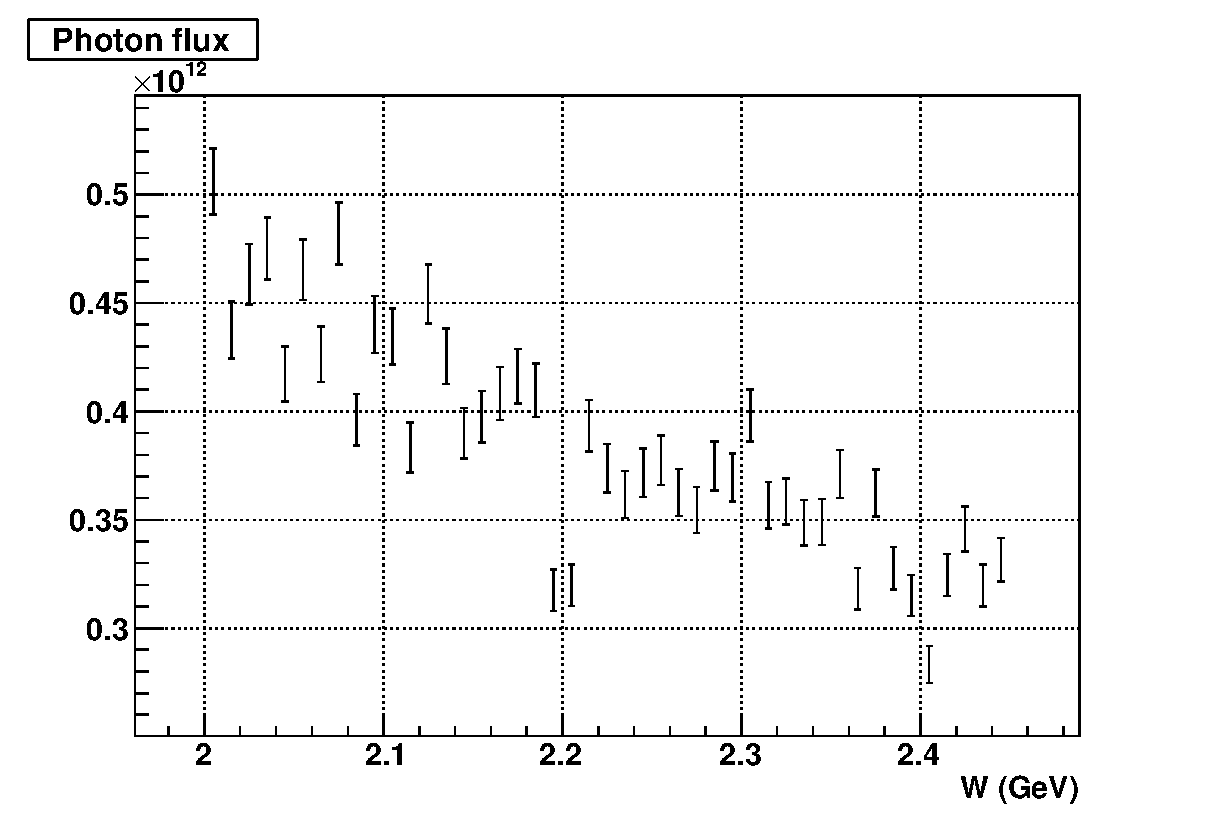
\includegraphics[width=.7 \textwidth]{xsec/flux.eps}
\caption{\label{fig:flux} The \textbf{corrected} photon flux incident on the target, as a function of $W$, together with the systematic error (3.04 $\%$).}
\end{figure}
\subsection{Results}

The two event yields (M.~Williams analysis / this analysis) are reported in Fig.\ref{fig:events}, left panel. The right panel reports the event yields ratio, as a function of $W$.
I decided to \textbf{not} quote any statistical or systematic error, since the two observables are extracted from the same dataset, using the same analysis procedure.
Instead, I decided to quote a $1\%$ systematic error to the M.~Williams results, due to the data digitization procedure (from the PhD thesis).

\begin{figure}[tpb]
\centering
\subfigure{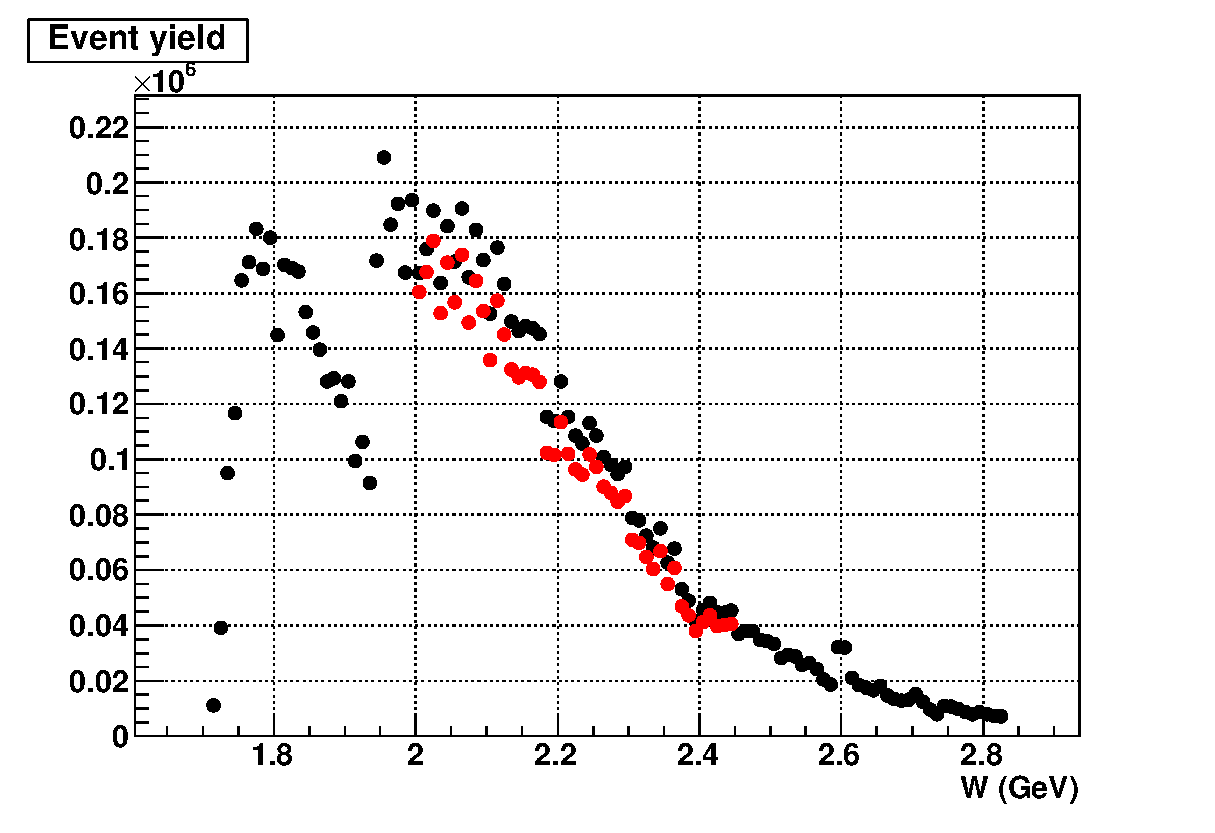
\includegraphics[width=.47 \textwidth]{xsec/events.eps}}
\subfigure{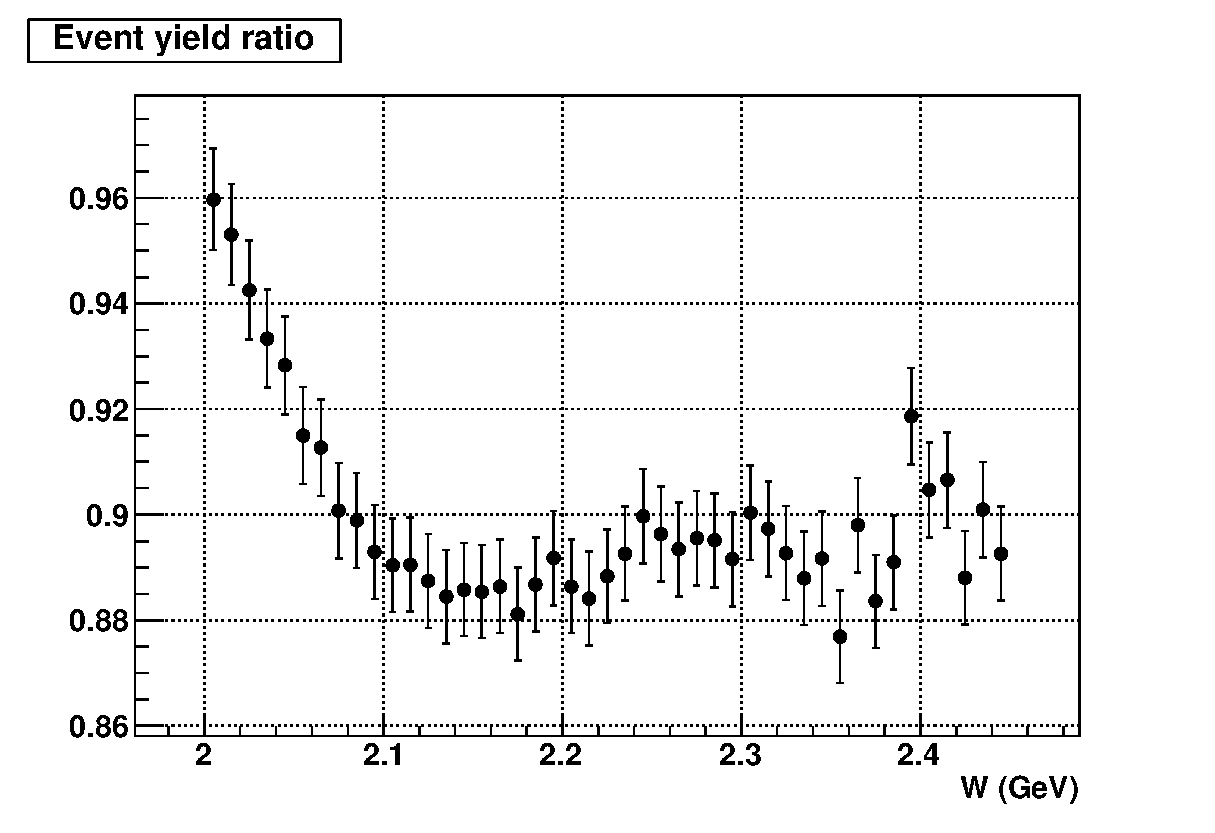
\includegraphics[width=.47 \textwidth]{xsec/eventsRatio.eps}}
\caption{\label{fig:events} Left: event yield as a function of $W$. Black: M.~Williams analysis (datapoints extracted from the PhD thesis). Red: this analysis.
Right: ratio of the two event yield, as a function of $W$. See text for the description of the error bars.}
\end{figure}


The result of the cross-section and spin-density matrix comparison is reported, for all $W$ bins, in appendix~\ref{Appendix:xsec}. In each page, the top-left plot reports the cross-section, while the central-row plots report the spin-density matrix elements, as a function of $\cos{\theta}_{CM}$.
The ratio between the two cross-sections is reported in the top-central plot. Results from M.~Williams analysis are reported in black, while results from this analysis are reported in red. 

\subsection{Conclusions}


\section{Effect of $F \neq 1$}

\subsection{Procedure}

\subsection{Results}

\subsection{Conclusions}






\begin{thebibliography}{99}
\bibitem{Szczepaniak:2014qca} 
  A.~P.~Szczepaniak and M.~R.~Pennington,
  %``Application of the Veneziano model to the analysis of three pion charmonium decays,''
  Phys.\ Lett.\ B {\bf 737}, 283 (2014).
  %%CITATION = PHLTA,B737,283;%%
  %2 citations counted in INSPIRE as of 31 Aug 2015
\bibitem{Williams:2009ab} 
  M.~Williams {\it et al.} [CLAS Collaboration],
  %``Differential cross sections and spin density matrix elements for the reaction gamma p ---> p omega,''
  Phys.\ Rev.\ C {\bf 80}, 065208 (2009)
  [arXiv:0908.2910 [nucl-ex]].
  %%CITATION = ARXIV:0908.2910;%%
  %38 citations counted in INSPIRE as of 31 Aug 2015
\bibitem{BrianCommunication}
  B.~Vernansky, private communication.

\bibitem{Williams:thesis}
M.~Williams. \textit{``Measurement of Differential Cross Sections and Spin Density Matrix Elements
along with a Partial Wave Analysis for $\gamma p \rightarrow p \omega$ using CLAS at Jefferson Lab.''} Ph.D.
thesis, Carnegie Mellon University, 2007.

\bibitem{Williams:2008ac} 
  M.~Williams, M.~Bellis and C.~A.~Meyer,
  %``Separating Signals from Non-Interfering Backgrounds using Probabilistic Event Weightings,''
  arXiv:0804.3382 [physics.data-an].
  %%CITATION = ARXIV:0804.3382;%%
  %2 citations counted in INSPIRE as of 31 Aug 2015

%chapter 2
\bibitem{Schilling:1969um} 
  K.~Schilling, P.~Seyboth and G.~E.~Wolf,
  %``On the Analysis of Vector Meson Production by Polarized Photons,''
  Nucl.\ Phys.\ B {\bf 15}, 397 (1970)
  [Nucl.\ Phys.\ B {\bf 18}, 332 (1970)].
  %%CITATION = NUPHA,B15,397;%%
  %212 citations counted in INSPIRE as of 31 Aug 2015

\bibitem{AmpTools}
H.~Matevosyan, R.~Mitchell and M.~Shepherd, \url{http://amptools.sourceforge.net/index.php/Main_Page}
\bibitem{gflux} J. Ball and E. Pasyuk. ``Photon Flux Determination Through Sampling of ”out-of-time” Hits
with the Hall B Photon Tagger.'' CLAS Note 2005-002.

\end{thebibliography}


\newpage







\appendix 
\section{Theorem}\label{app:theo}
\begin{theorem}
\printteolike
\end{theorem}







\section{Data agreement with previous results: plots}\label{Appendix:xsec}
%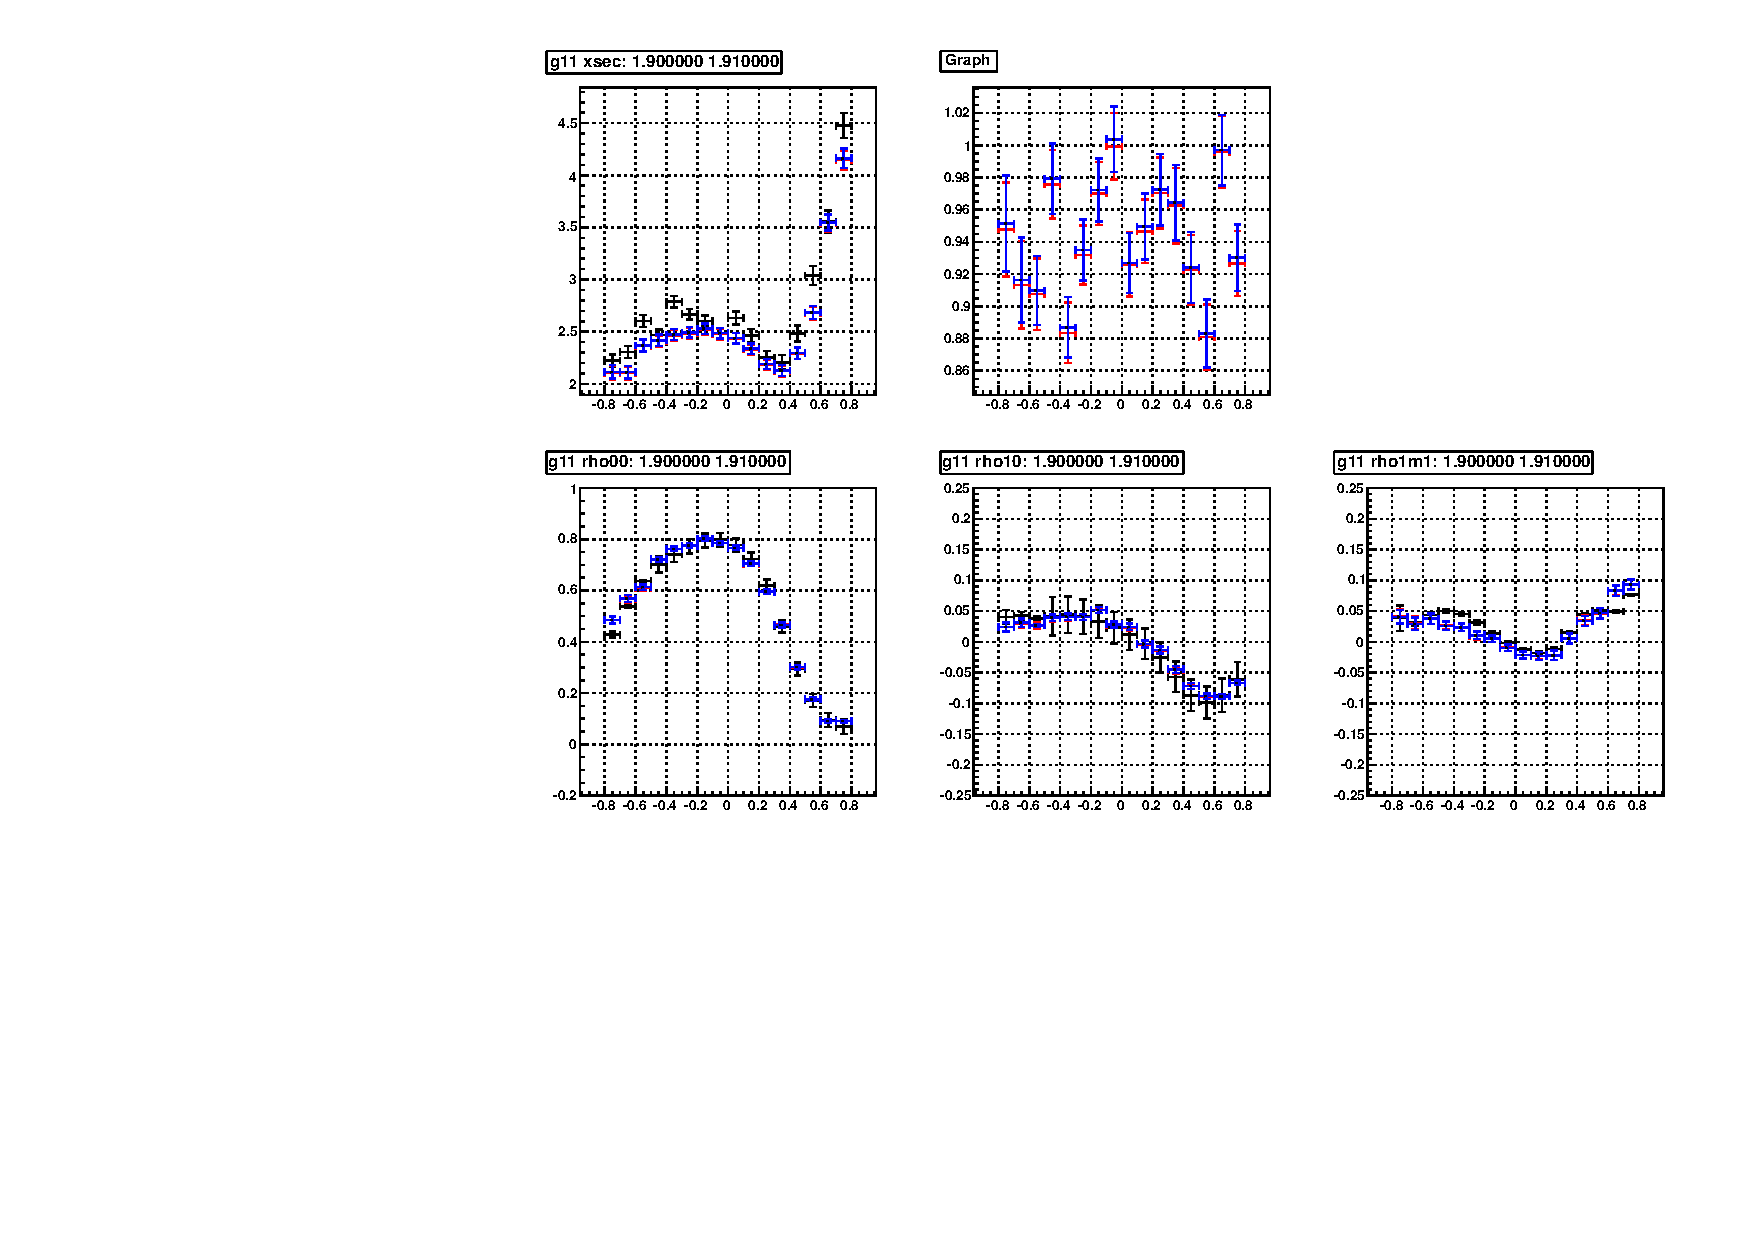
\includepdf[pages={1-},scale=0.75]{out.pdf}

\forloop[1]{counter}{1}{\value{counter} < 45}{%
%
%\ifnum\value{counter} = 5
%Bin 5 : $W=$ 1.95-1.96 GeV is excluded from the analysis
%
%\else
\includegraphics[width=\textwidth]{xsec/xsec_\arabic{counter}.eps}
\centering
Bin
\bind{S}{\value{counter}}
: $W= $
\use[2]{ S * 0.01+2.0} - \use[2]{ S * 0.01+2.01} GeV
\newpage
}%








\end{document}